\section{Causes of Evolvability: Intuition}

\begin{frame}{Summary}
  \alert{big idea}: internal system configuration determines the outcomes of change to the system
\end{frame}


\begin{frame}{Computer Science Intuition: Spaghetti Code}
  idea: software without compartmentalization, error handling, with hard-coded constants, etc. is much more difficult to alter in useful ways
  \begin{figure}
  \centering
  \begin{subfigure}[b]{0.5\textwidth}
    \centering
    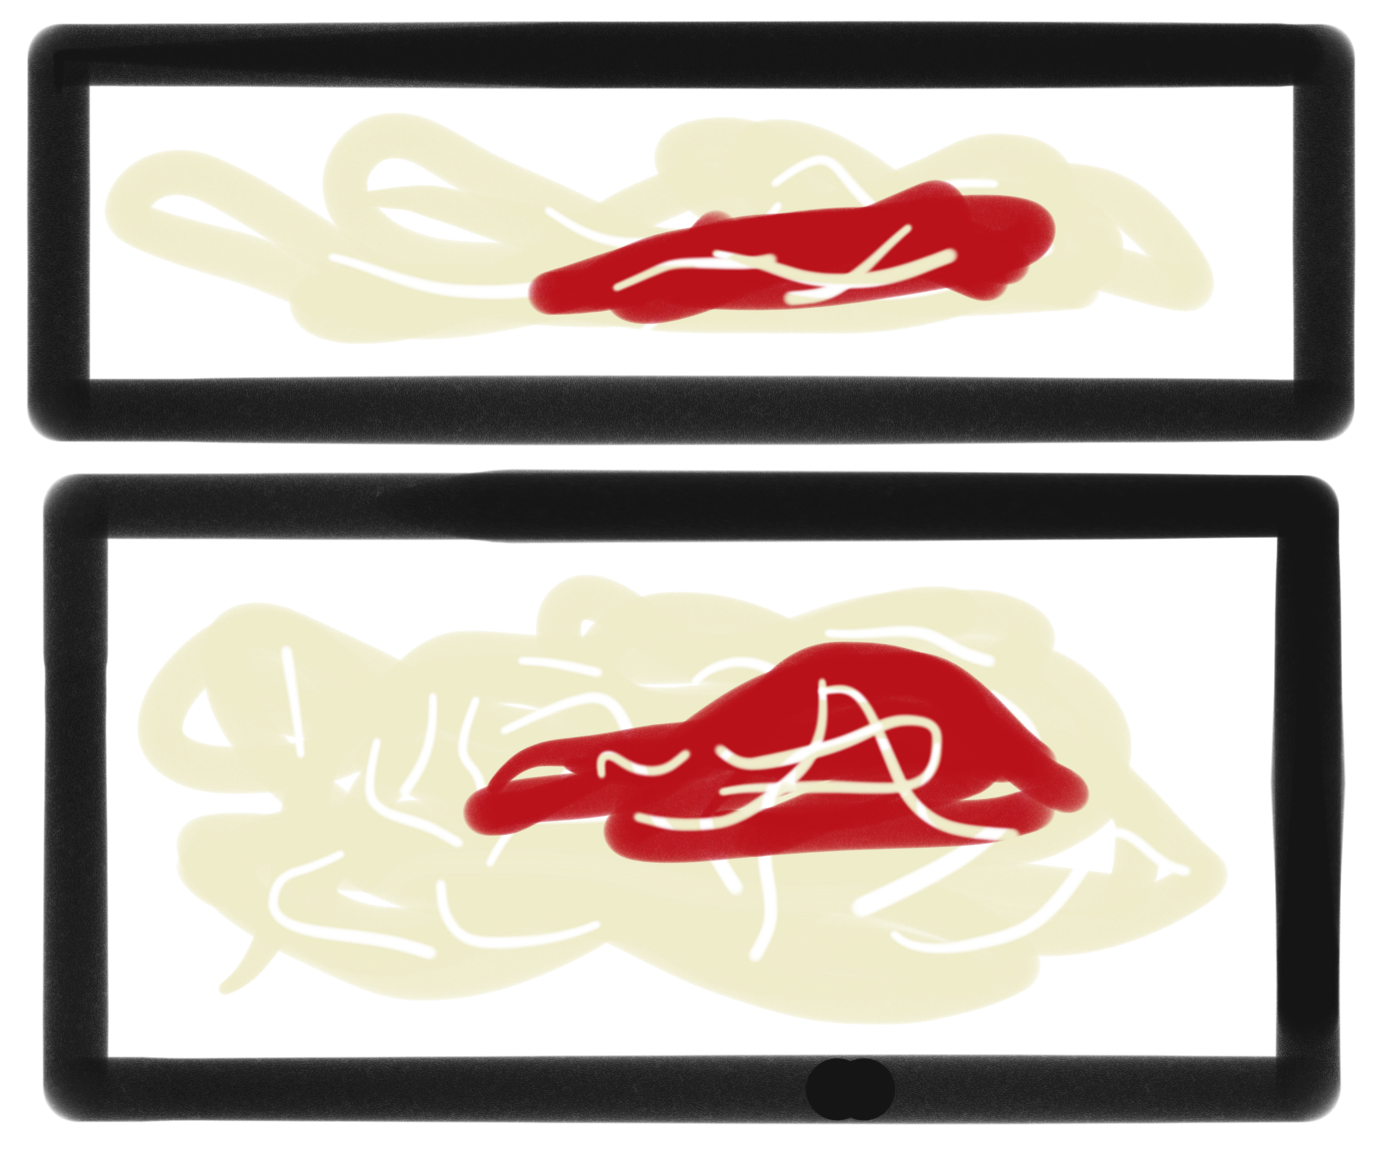
\includegraphics[width=\textwidth]{img/spaghetticode}
    \caption{spaghetti code}
    \label{subfig:spaghetti_code}
  \end{subfigure}%
  \hfill
  \begin{subfigure}[b]{0.5\textwidth}
    \centering
    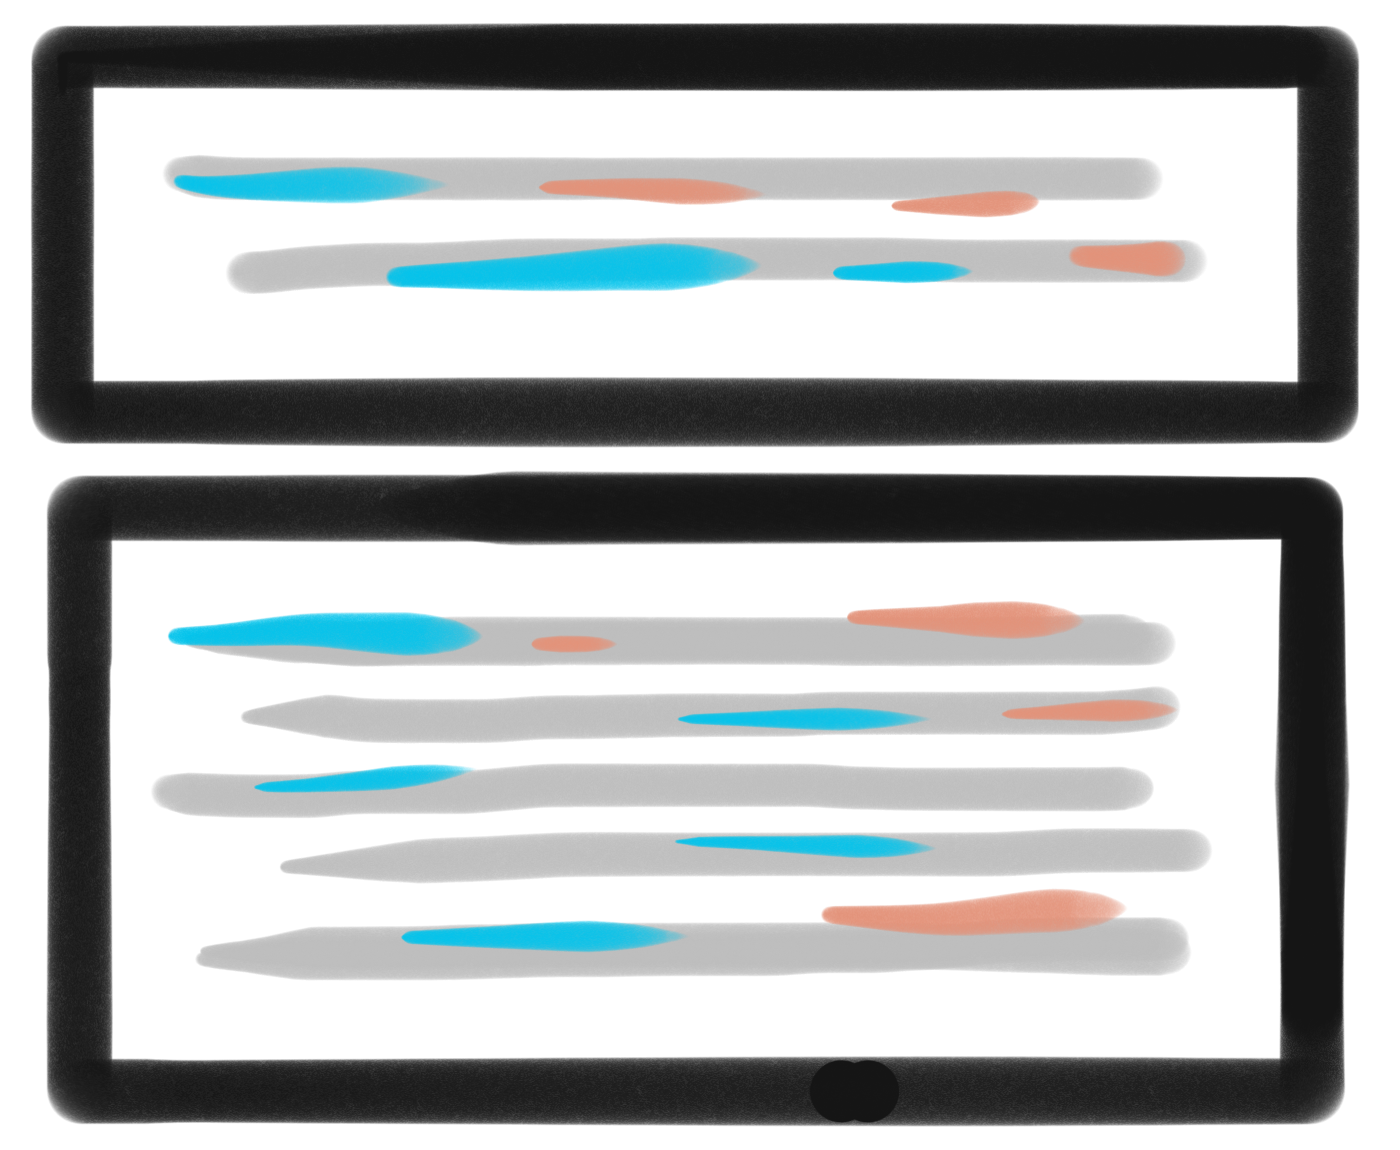
\includegraphics[width=\textwidth]{img/regularcode}
    \caption{regular code}
     \label{subfig:regular_code}
  \end{subfigure}
  \captionsetup{singlelinecheck=off,justification=raggedright}
  \caption{A cartoon comparison of spaghetti and regular code.}
  \label{fig:direct_irregular_vs_indirect_regular}
\end{figure}
\end{frame}

\begin{frame}{Computer Science Intuition: Spaghetti Code}
  idea: software without compartmentalization, error handling, with hard-coded constants, etc. is much more difficult to alter in useful ways
  \begin{figure}
  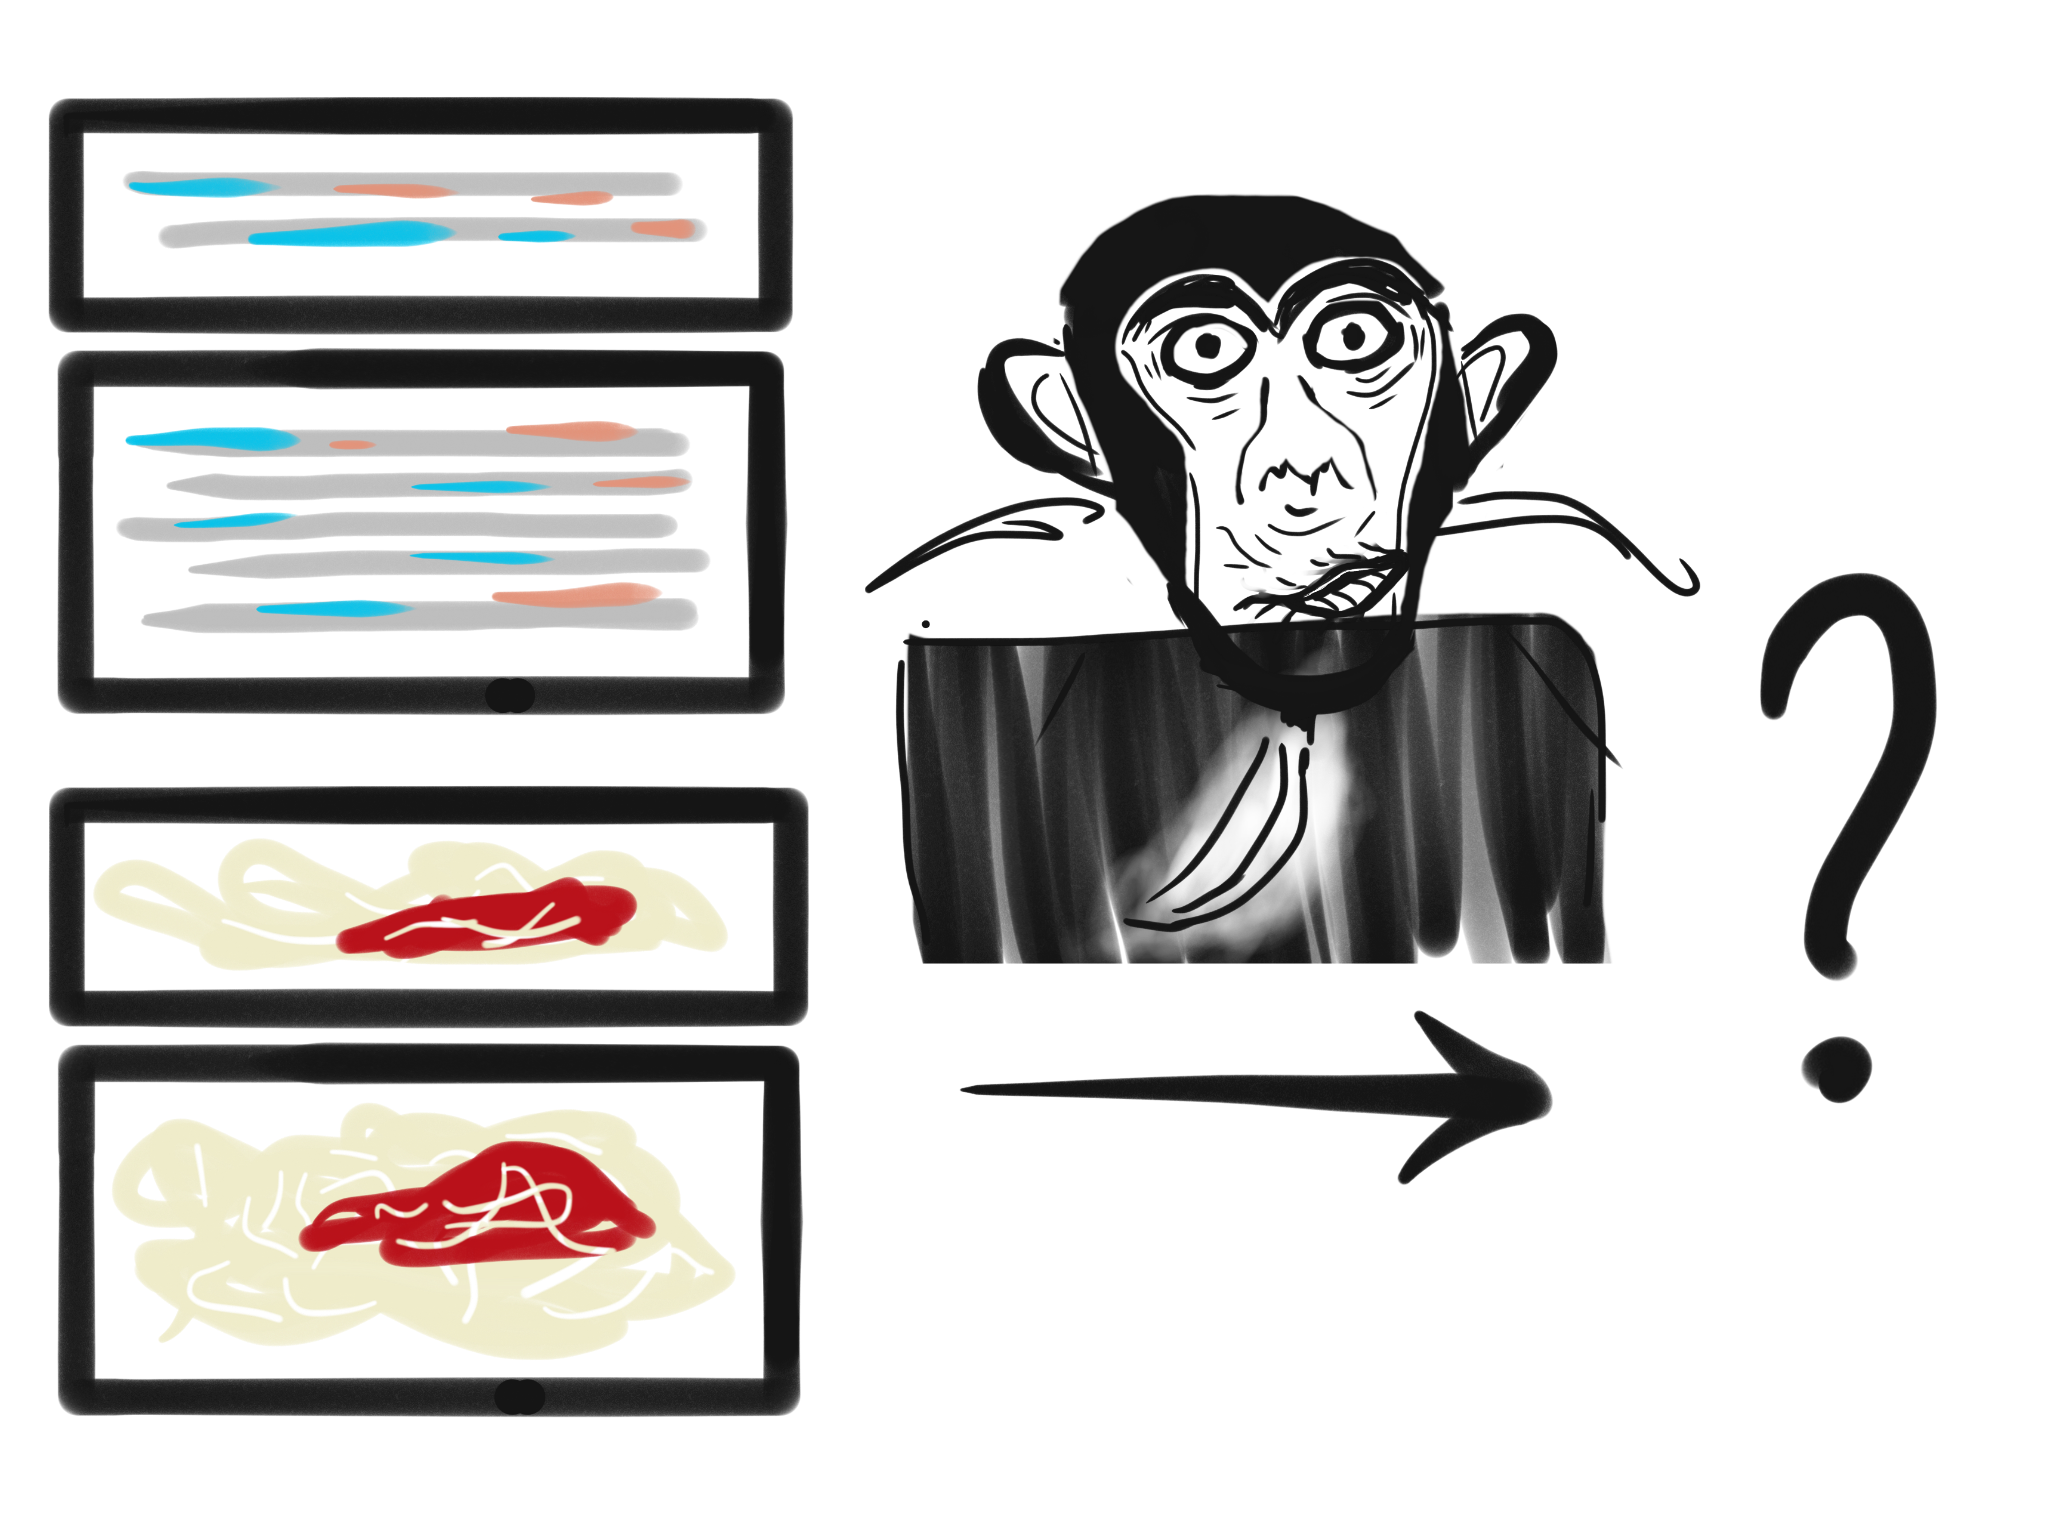
\includegraphics[width=0.6\textwidth]{img/spaghetti_monkey}
  \captionsetup{singlelinecheck=off,justification=raggedright}
  \caption{Spaghetti code and proper code might experience different distributions of outcomes from arbitrary changes to the software made by a junior developer from the local primate house.}
\end{figure}
\end{frame}

\begin{frame}{Biological Perspective: Intraindividual Degeneracy}
  idea: employing a diverse collection of substructures that provide identical or near-identical functionality promote robustness through redundancy while providing many jumping off points for variation through repurposing or elaboration
  \begin{figure}
 \begin{columns}
 \begin{column}{0.6\textwidth}
 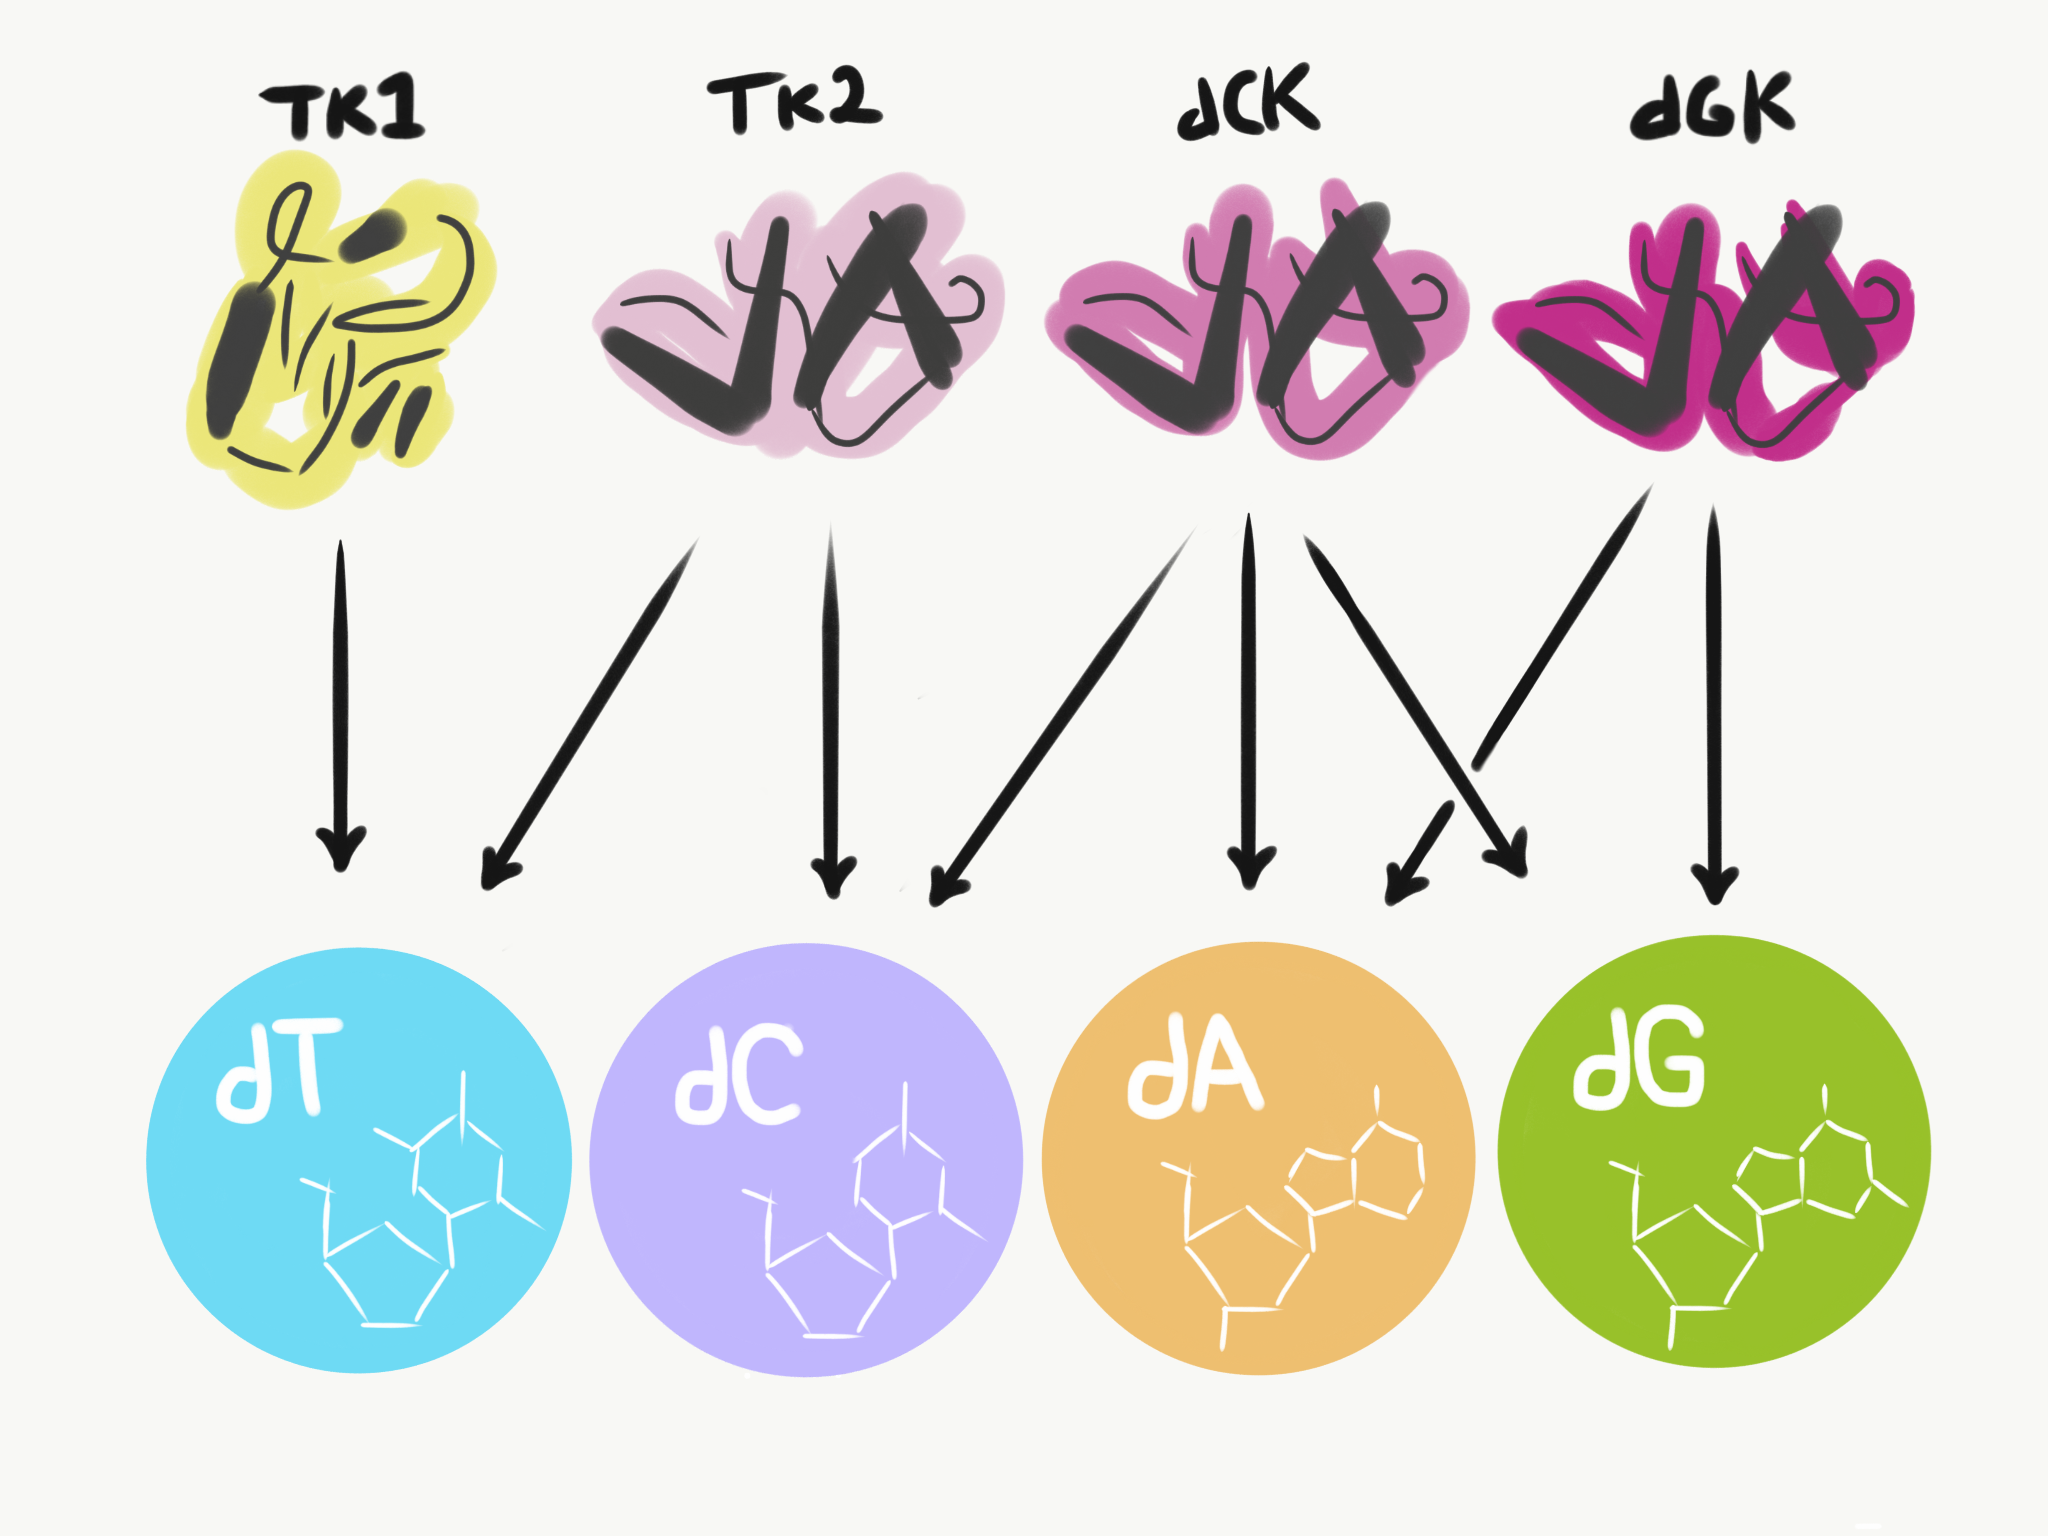
\includegraphics[width=\textwidth]{img/intraindividual_degeneracy}
 \end{column}
 \begin{column}{0.4\textwidth}
\captionsetup{singlelinecheck=off,justification=raggedright}
  	\caption{Mammalian deoxyribonucleoside kinases exhibit degeneracy \cite{Sandrini2005DeoxyribonucleosideReaction.}.}
    \label{fig:intraindividual_degeneracy}
    
\end{column}
\end{columns}
\end{figure}
\end{frame}
